\chapter{Selected Validation Evidence}
\label{app:validation-evidence}

This appendix presents the eight retained interface captures supplied for the report. They were collected at different moments of the validation campaign rather than as one synchronized snapshot. Each figure supports only the indicators stated in its caption; the final architecture and validation boundaries remain those documented in Chapters~VI--VIII.

\begingroup
\captionsetup[figure]{font=footnotesize}

\section{Orchestration and Quality Evidence}

\begin{figure}[H]
    \centering
    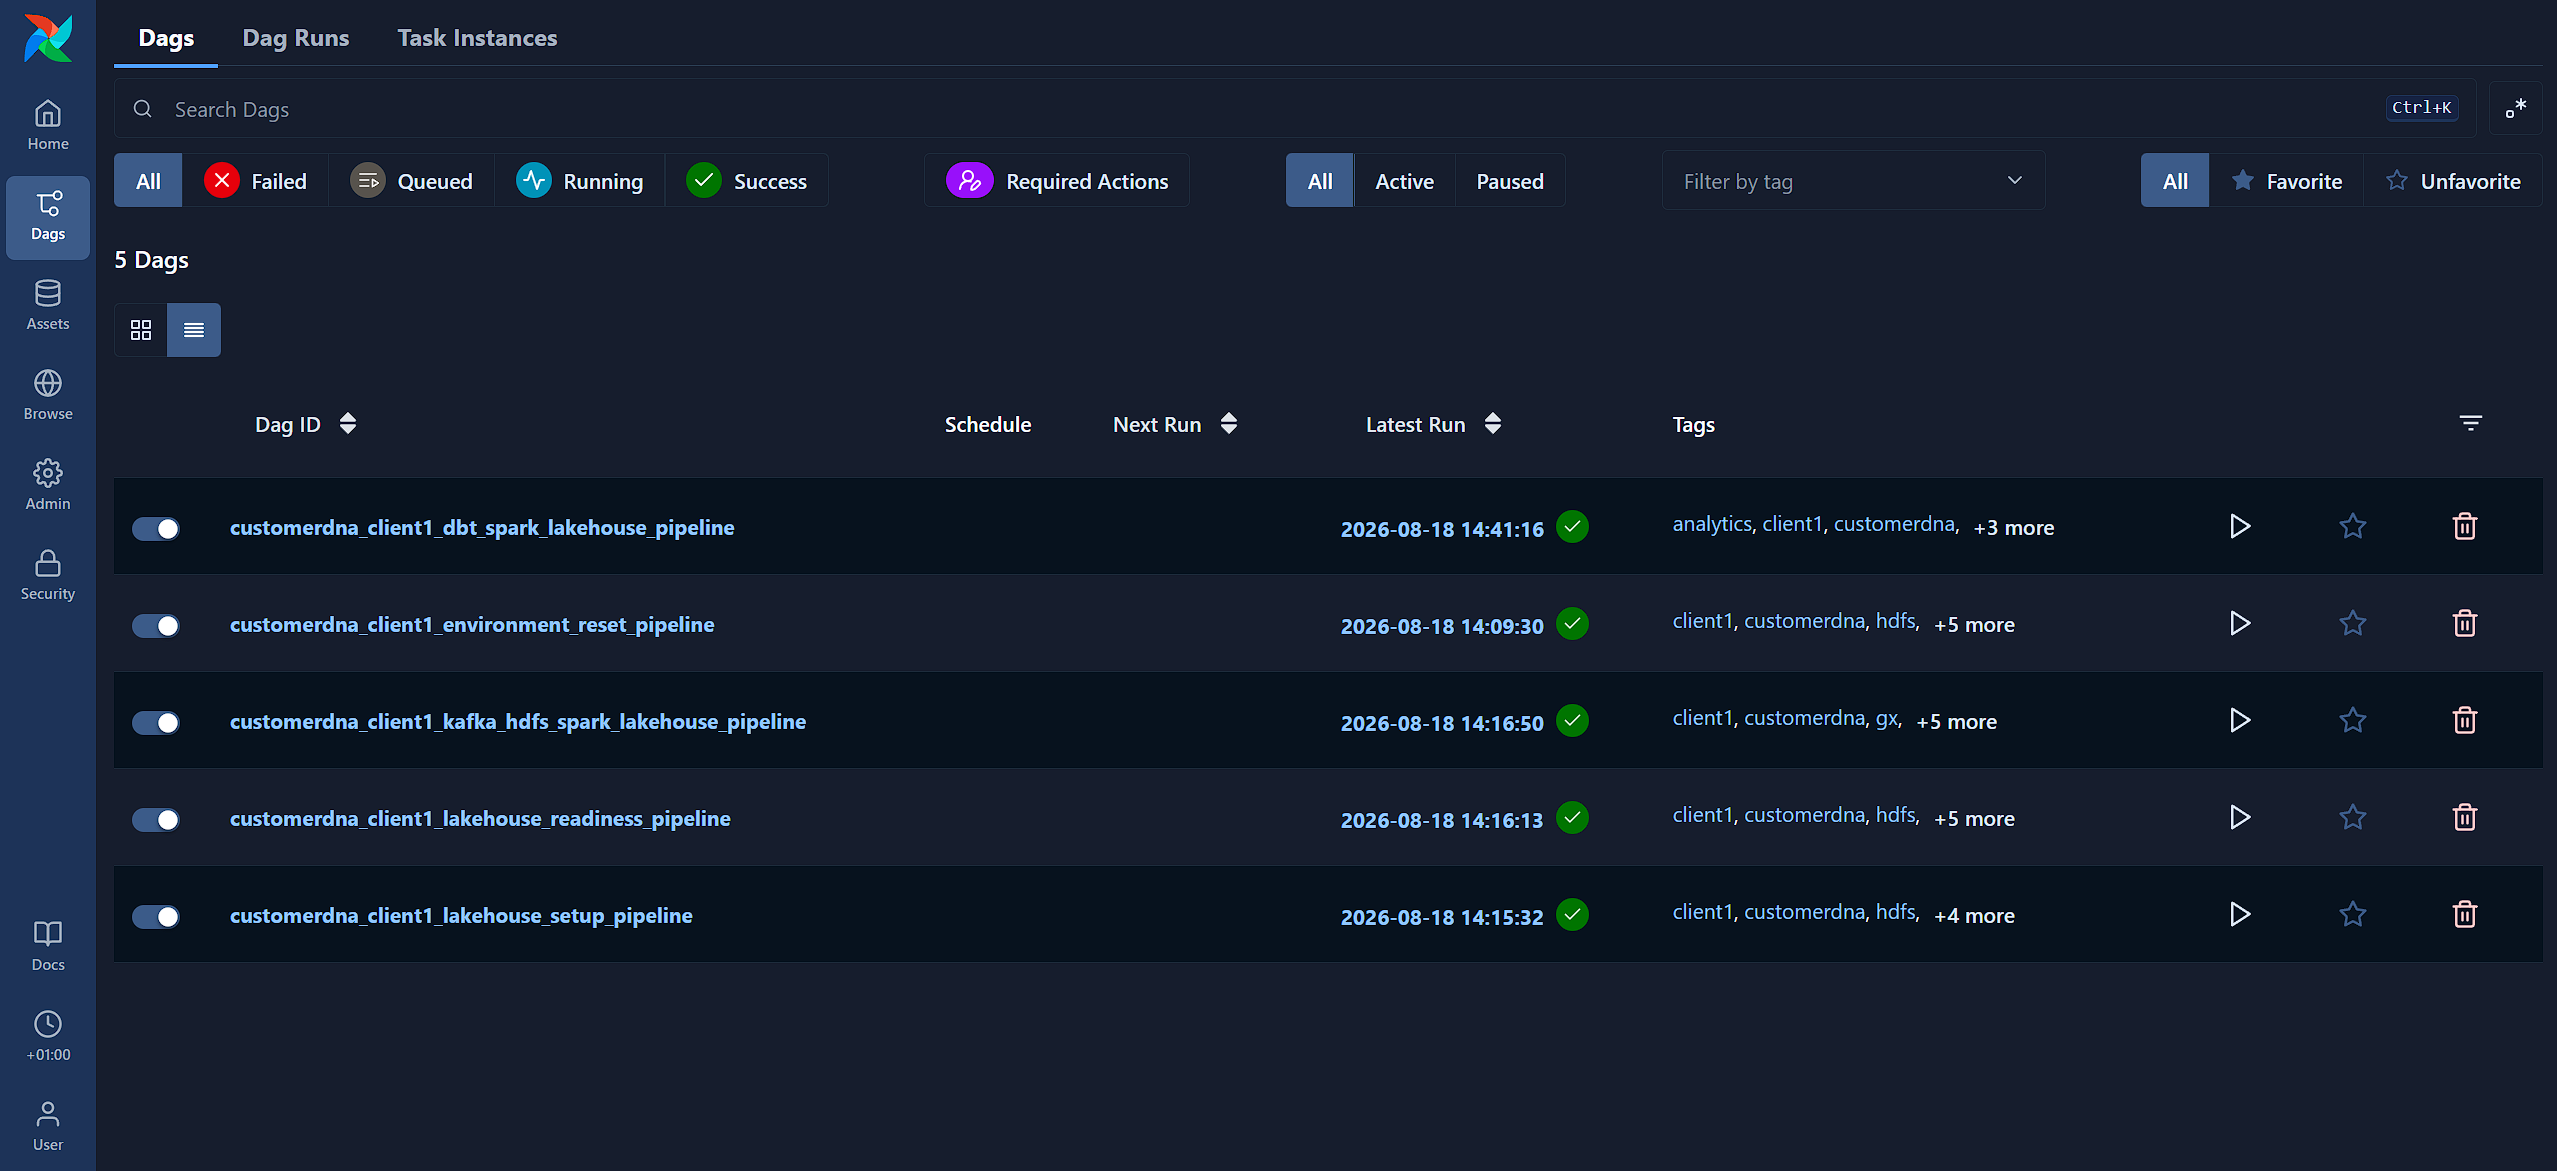
\includegraphics[
        viewport=75 143 1238 706,
        clip,
        width=\textwidth,
        keepaspectratio
    ]{91_evidence/airflow_success.png}
    \captionsetup{font=small}
    \caption[Airflow workflow execution evidence]{Airflow grid captured on August 18, 2026, showing successful latest runs for the five implemented workflows: environment reset, lakehouse setup, lakehouse readiness, Kafka--HDFS--Spark raw loading with integrated raw-quality tasks, and dbt-spark transformation.}
    \label{fig:appendix-airflow-runs}
\end{figure}

\clearpage
\begin{landscape}
    \thispagestyle{plain}
    \vspace*{1cm}
    \begin{figure}[H]
        \centering
        \makebox[\linewidth][c]{%
            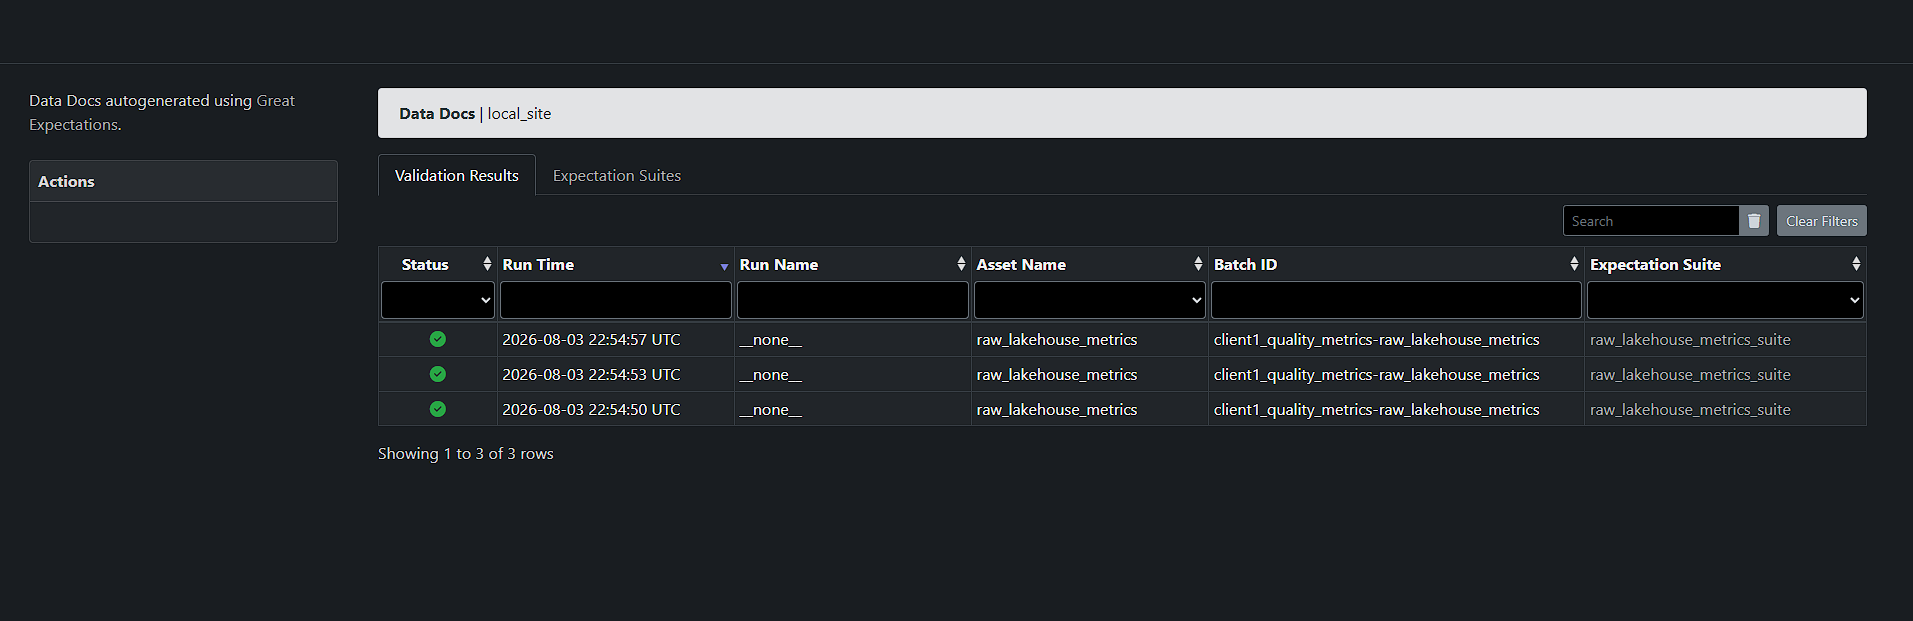
\includegraphics[
                viewport=263 125 1418 414,
                clip,
                width=0.98\linewidth,
                keepaspectratio
            ]{91_evidence/great_expectations_data_docs.png}%
        }
        \captionsetup{font=small,width=0.96\linewidth}
        \caption[Great Expectations Data Docs evidence]{Great Expectations Data Docs showing three successful raw-lakehouse validation records retained on August 3, 2026.}
        \label{fig:appendix-gx-docs}
    \end{figure}
    \vspace*{\fill}
\end{landscape}
\clearpage

\begin{landscape}
    \thispagestyle{plain}
    \section{Observability Evidence}
    \vspace*{\fill}
    \begin{figure}[H]
        \centering
        \makebox[\linewidth][c]{%
            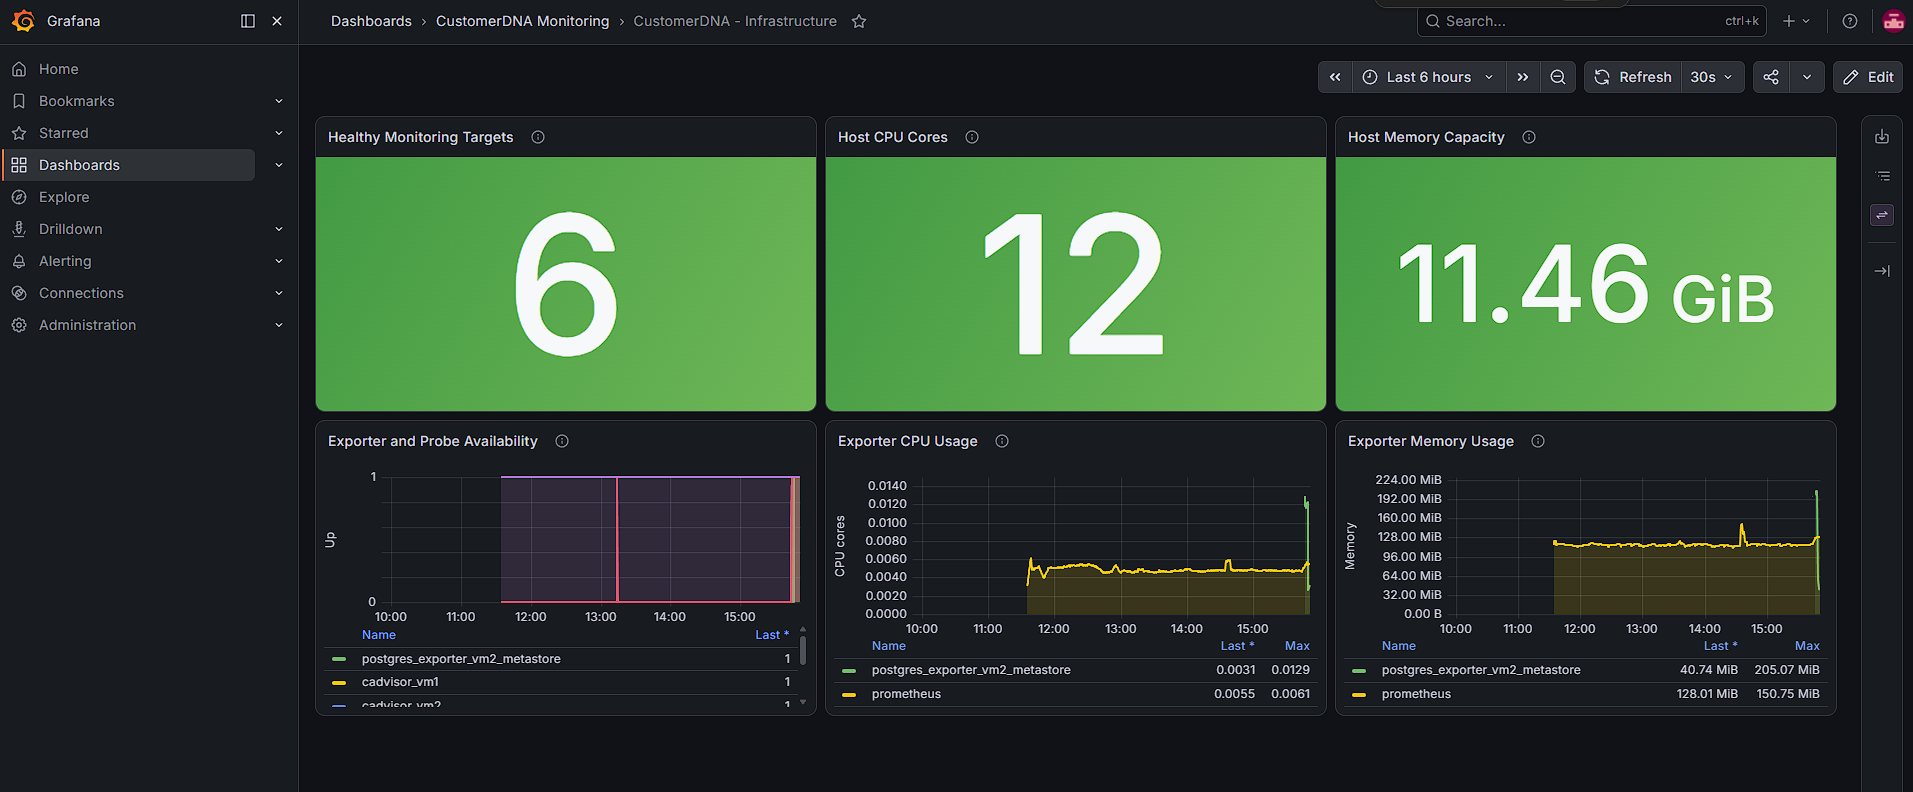
\includegraphics[
                viewport=225 50 1380 519,
                clip,
                width=0.98\linewidth,
                keepaspectratio
            ]{91_evidence/grafana_dashboard_infrastructure.png}%
        }
        \captionsetup{font=small,width=0.96\linewidth}
        \caption[Grafana infrastructure monitoring evidence]{Grafana infrastructure overview showing six healthy monitoring targets, twelve observed CPU cores, 11.46~GiB of host memory, and the associated availability and utilization panels.}
        \label{fig:appendix-infrastructure-dashboard}
    \end{figure}
    \vspace*{\fill}
\end{landscape}
\clearpage

\begin{landscape}
    \thispagestyle{plain}
    \vspace*{\fill}
    \begin{figure}[H]
        \centering
        \makebox[\linewidth][c]{%
            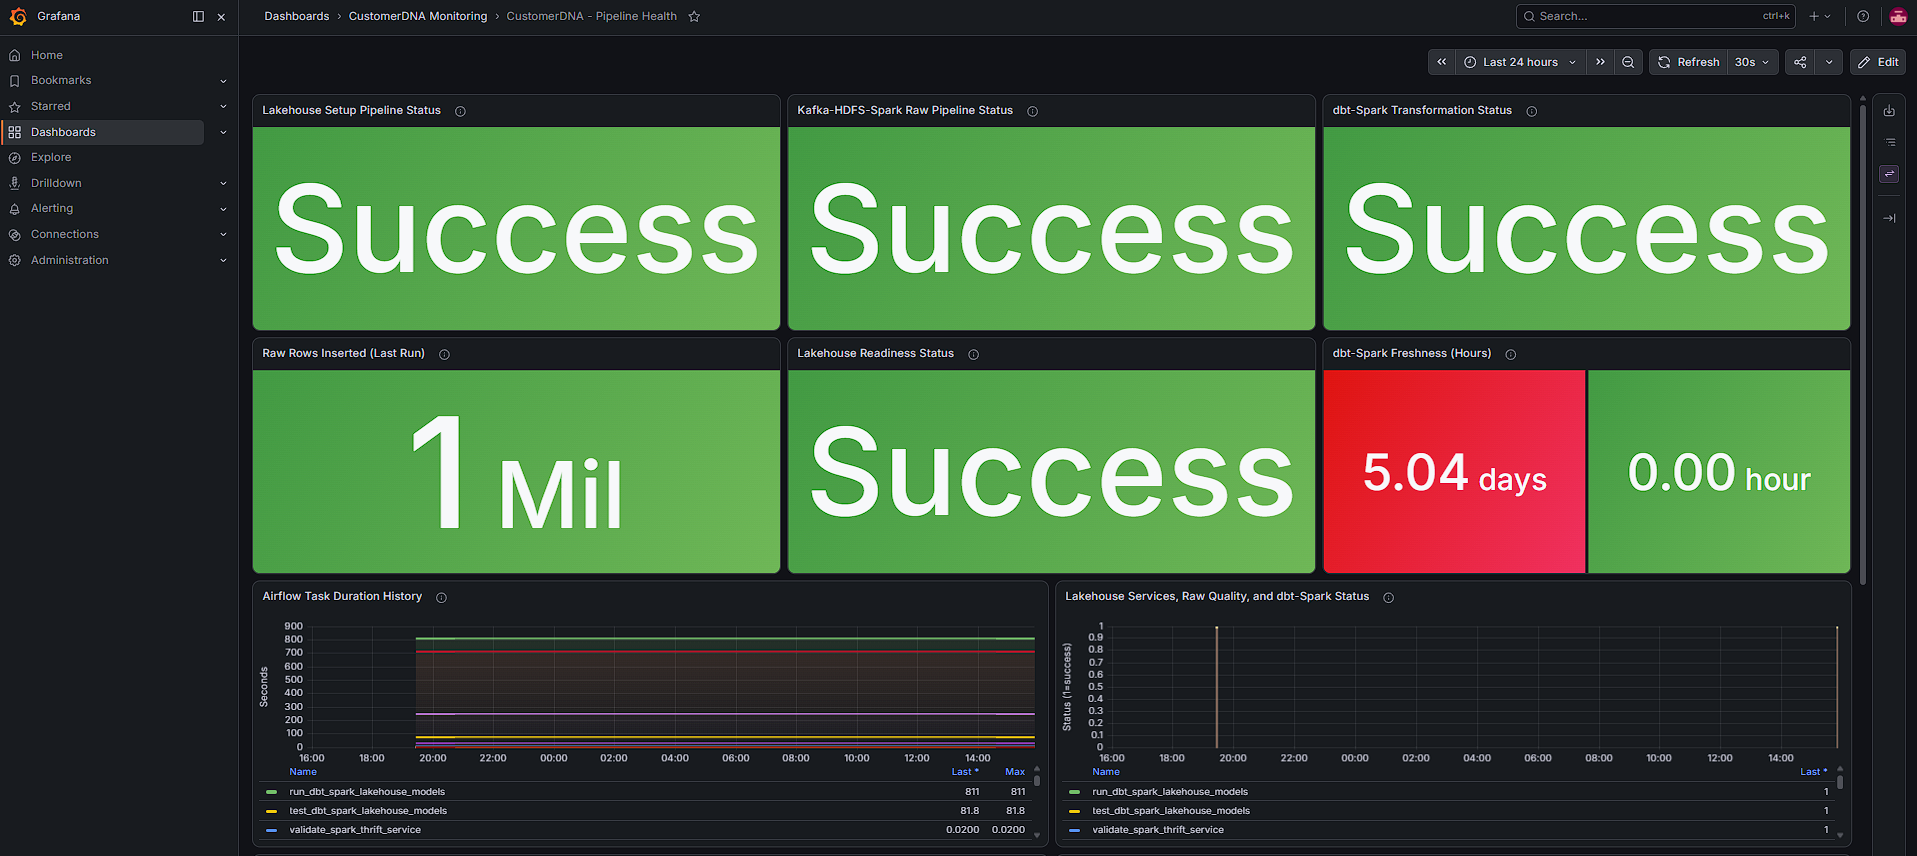
\includegraphics[
                viewport=184 5 1391 575,
                clip,
                width=0.98\linewidth,
                keepaspectratio
            ]{91_evidence/grafana_dashboard_pipeline_health.png}%
        }
        \captionsetup{font=small,width=0.96\linewidth}
        \caption[Grafana pipeline-health evidence]{Grafana pipeline-health view retaining workflow status, raw-row volume, readiness, and freshness indicators as they appeared at the dashboard capture time.}
        \label{fig:appendix-pipeline-dashboard}
    \end{figure}
    \vspace*{\fill}
\end{landscape}
\clearpage

\begin{landscape}
    \thispagestyle{plain}
    \section{Storage and Metadata Evidence}
    \vspace*{\fill}
    \begin{figure}[H]
        \centering
        \makebox[\linewidth][c]{%
            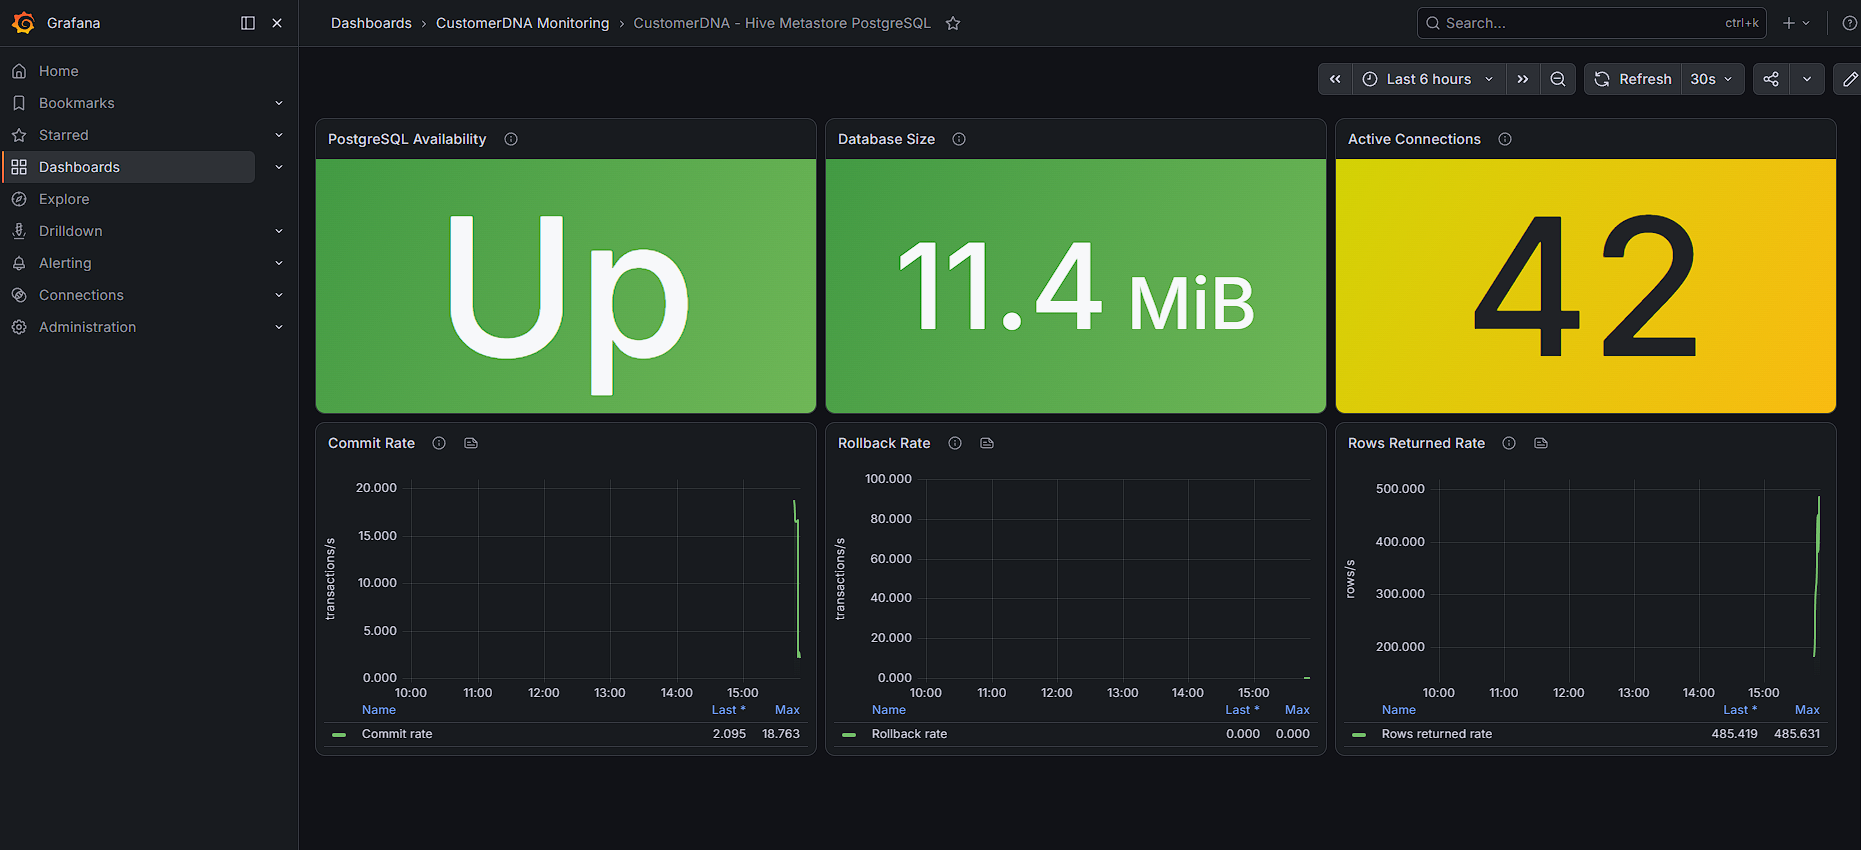
\includegraphics[
                viewport=214 11 1358 555,
                clip,
                width=0.98\linewidth,
                keepaspectratio
            ]{91_evidence/grafana_dashboard_hive_metastore.png}%
        }
        \captionsetup{font=small,width=0.96\linewidth}
        \caption[Grafana Hive Metastore monitoring evidence]{Grafana Hive Metastore dashboard showing PostgreSQL availability, a database size of 11.4~MiB, 42 active connections in this time-specific capture, and transaction and row-return activity.}
        \label{fig:appendix-hive-dashboard}
    \end{figure}
    \vspace*{\fill}
\end{landscape}
\clearpage

\vspace*{\fill}
\begin{figure}[H]
    \centering
    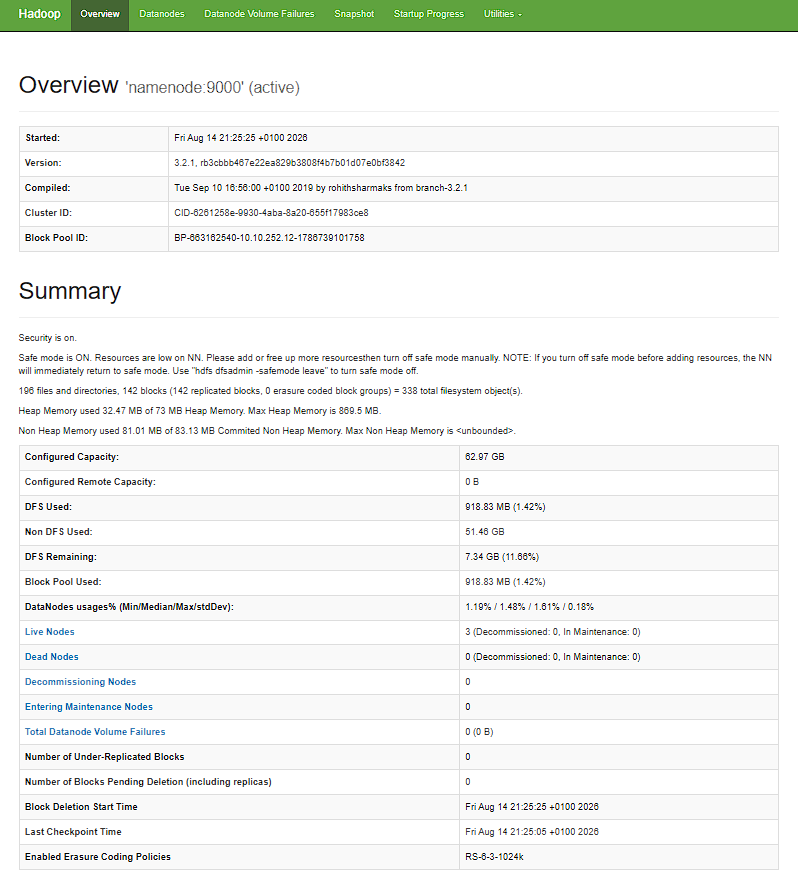
\includegraphics[
        viewport=11 5 585 661,
        clip,
        width=\textwidth,
        height=0.78\textheight,
        keepaspectratio
    ]{91_evidence/hdfs_cluster_health.png}
    \captionsetup{font=small}
    \caption[HDFS cluster-capacity and DataNode evidence]{HDFS administrative overview showing 62.97~GB of configured capacity, three live DataNodes, no dead nodes, and no under-replicated blocks. The visible security and safe-mode notices are not used as evidence for the final hardened access path.}
    \label{fig:appendix-hdfs-health}
\end{figure}
\vspace*{\fill}
\clearpage

\begin{landscape}
    \thispagestyle{plain}
    \section{Distributed Processing and Analytical Access}
    \vspace*{\fill}
    \begin{figure}[H]
        \centering
        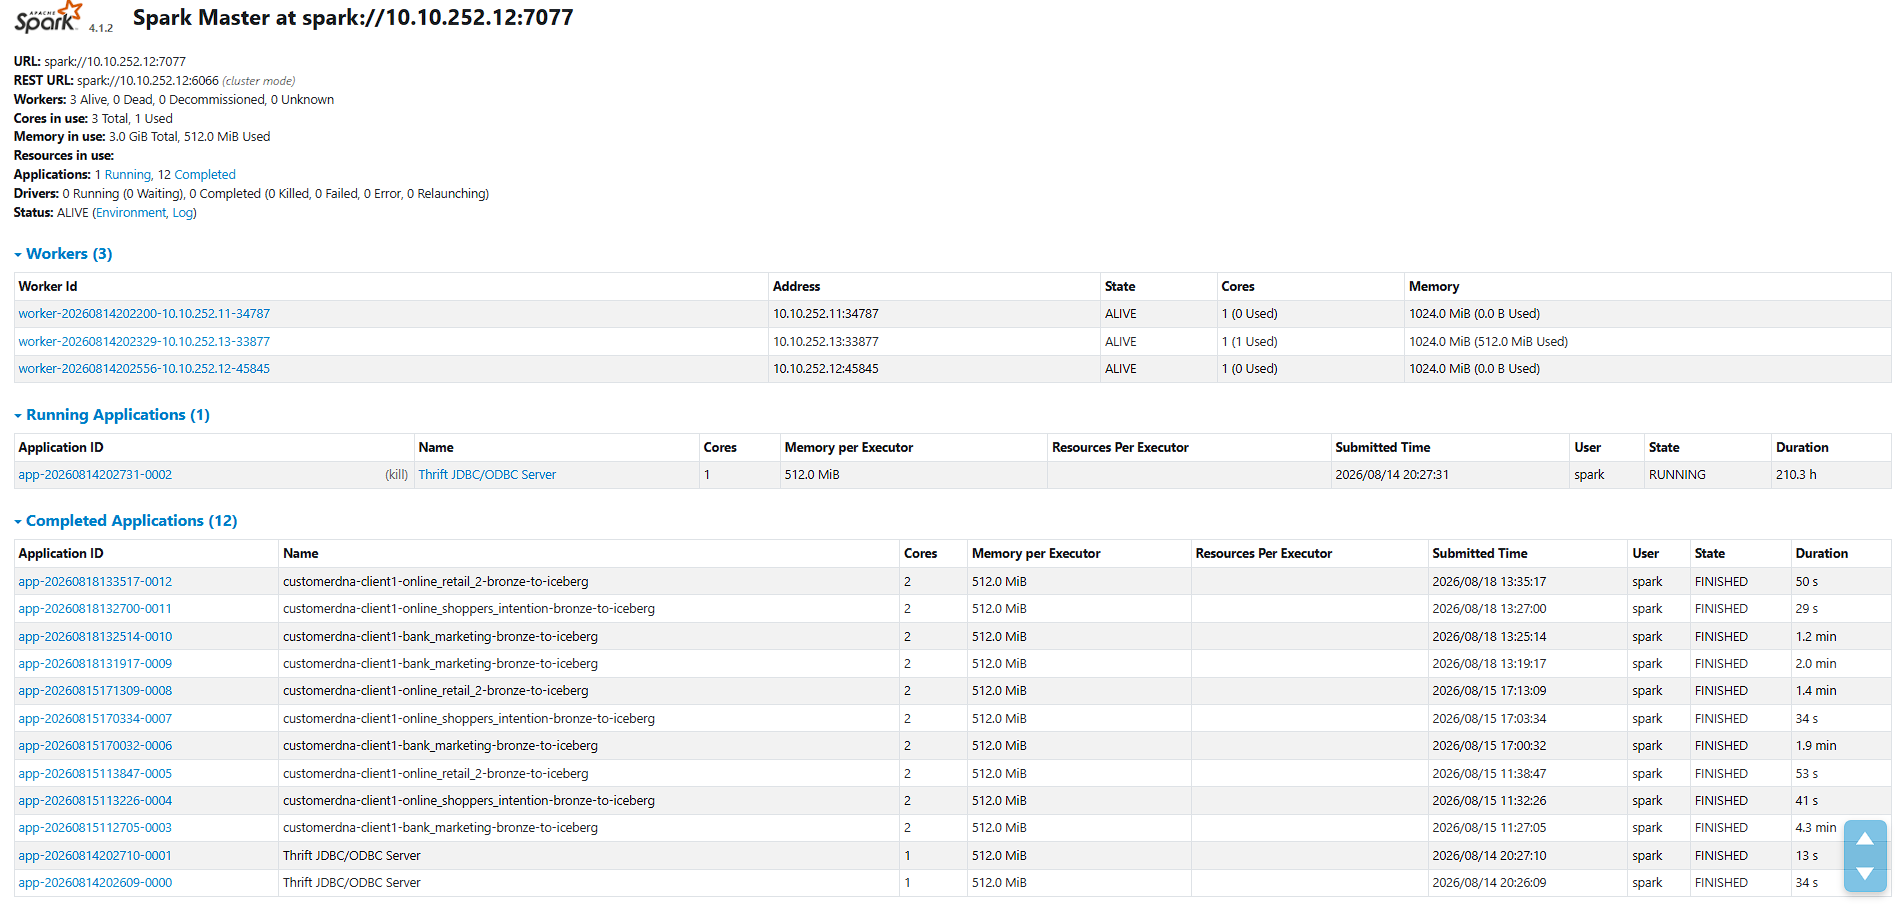
\includegraphics[
            viewport=8 6 1421 677,
            clip,
            width=0.98\linewidth,
            keepaspectratio
        ]{91_evidence/spark_cluster_workers.png}
        \captionsetup{font=small,width=0.96\linewidth}
        \caption[Spark worker and application evidence]{Spark master interface showing three alive workers, three aggregate cores, 3.0~GiB of worker memory, an active Thrift JDBC/ODBC service, and twelve completed applications.}
        \label{fig:appendix-spark-workers}
    \end{figure}
    \vspace*{\fill}
\end{landscape}
\clearpage

\begin{landscape}
    \thispagestyle{plain}
    \vspace*{\fill}
    \begin{figure}[H]
        \centering
        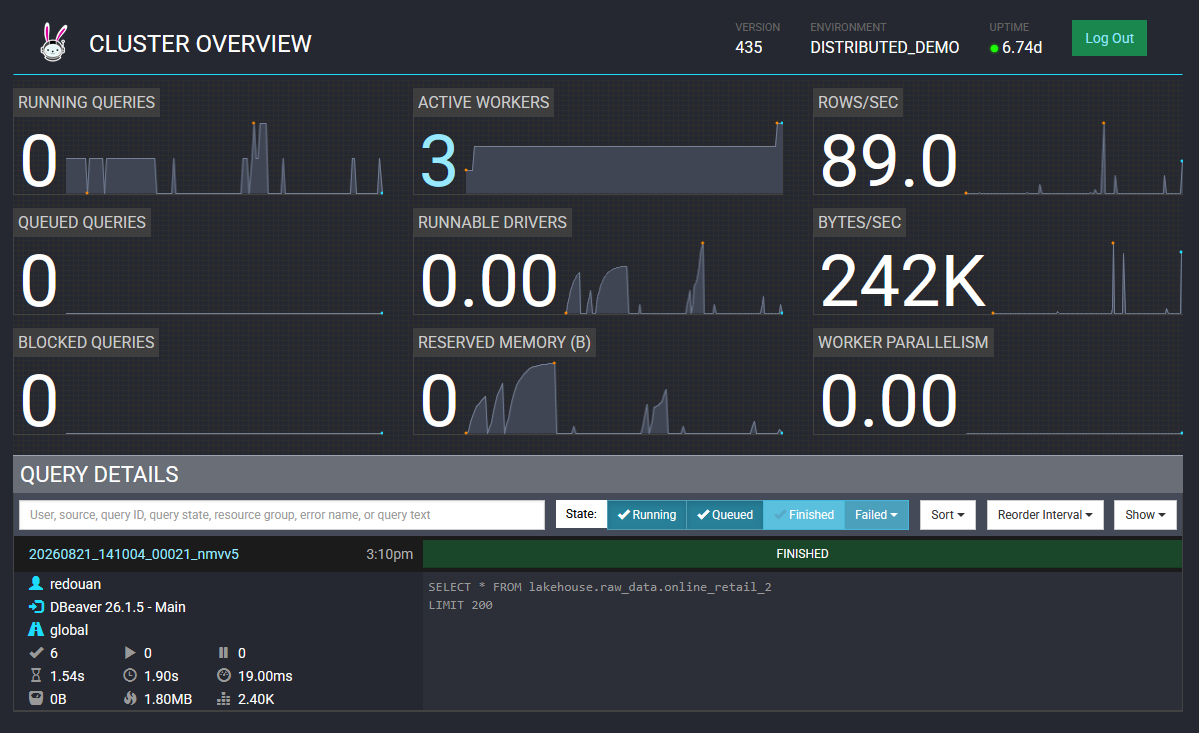
\includegraphics[
            viewport=10 18 1185 728,
            clip,
            width=0.94\linewidth,
            keepaspectratio
        ]{91_evidence/trino_query_result.png}
        \captionsetup{font=small,width=0.92\linewidth}
        \caption[Trino cluster and completed-query evidence]{Trino 435 cluster view showing environment \texttt{DISTRIBUTED\_DEMO}, 6.74 days of uptime, three active execution nodes, and a completed query over \path{lakehouse.raw_data.online_retail_2} with the displayed throughput snapshot.}
        \label{fig:appendix-trino-query}
    \end{figure}
\end{landscape}
\endgroup